

\documentclass[10pt]{beamer}

\linespread{1.0}

\usetheme{Pittsburgh}
%\usetheme {CambridgeUS}%{Goettingen}%{Berkeley}%{Montpellier}%{Antibes}%{Dresden}%{Madrid}%{Dresden}%{Darmstadt}%{Warsaw}%{Pittsburgh}
\usefonttheme{serif}%{structurebold}%{structuresmallcapsserif}%{professionalfonts}
\usepackage[english]{babel}
%\usepackage[latin1]{inputenc}
\usepackage{hyperref}
%\usecolortheme{beaver}
%\usecolortheme{crane}

\setbeamercovered{transparent}


\usepackage{latexsym}
\usepackage{amsmath}
\usepackage{times}
\usepackage{MinionPro}
\usepackage{hyperref}
\usepackage{tikz}
\usepackage{verbatim}
\usepackage{natbib}
\usepackage{color, colortbl}
\usepackage{appendix}
\usepackage{ulem}
\usepackage{amsmath,amsthm}

\usetikzlibrary{arrows,shapes}


\newtheorem{proposition}{Proposition}[section]
%\newtheorem{definition}{Definition}[section]
\newtheorem{assumption}{Assumption}[section]
\newtheorem{conjecture}{Conjecture}[section]



\definecolor{Gray}{gray}{0.9}


\pgfdeclarelayer{background}
\pgfsetlayers{background,main}

\tikzstyle{vertex}=[circle,fill=black!25,minimum size=12pt,inner sep=0pt]
\tikzstyle{selected vertex} = [vertex, fill=red!24]
\tikzstyle{unknown vertex} = [vertex, fill=black]
\tikzstyle{edge} = [draw,thick,-]
\tikzstyle{weight} = [font=\small]
\tikzstyle{selected edge} = [draw,line width=5pt,-,red!50]
\tikzstyle{ignored edge} = [draw,line width=5pt,-,black!20]



\setbeamercovered{transparent}




\title{Coordination in Social Networks}
\author{Chun-ting Chen}


\begin{document}

\maketitle


\section{Introduction}
\subsection{Motivation}

\frame{
  \frametitle{Motivation}
  
\begin{itemize}

\item Consider a rigid regime, where ``communication barrier'' is imposed to impede people to show their discontents.
\item {Communication barrier}
\begin{enumerate}
\item Threatened by suppression, exile, eavesdropping, etc.
\item No (fair) voting system, No (fair) mass media, No (uncensored) discussion forum, etc.

\end{enumerate} 
\item \textit{How do Rebels made decisive collective action?}

\end{itemize}  
  
}

\frame{
  \frametitle{Motivation}
History tells us:

\begin{itemize}

\item An event may trigger later events.
\begin{itemize}
\item Benny Tai, a leader of Occupy Central, has said \textit{``It (Umbrella Protest) is beyond what I imagined''}, while Occupy Central trigger the  Umbrella Protest in Hong Kong.
\end{itemize}

\item People communicate in their social network.
\begin{itemize}
\item Ex., Gangster networks (1911 Revolution); Church networks (1989 Berlin Uprising, 2014 Umbrella Protest ); Friend networks, etc.
\end{itemize}



\end{itemize}  
  
}

\frame{
  \frametitle{Motivation}

Question  
  \begin{itemize}
  \item \textit{If rational rebels know that a ``tiny'' event can trigger later events, how do they conduct a revolution under communication barrier?}
  \end{itemize}
  
Objective  
\begin{itemize}
\item What kinds of social networks can conduct such decisive collective action?
\end{itemize}

Model 
\begin{enumerate}
\item Rebels communicate in network.
\item Communication is not free but costly.
\item Communication is through taking actions.
\end{enumerate}





}




\frame{
  \frametitle{Motivation}

Looking for 
\begin{itemize}

\item An equilibrium, where the ex-post efficient outcome played repeatedly after a finite time $T$ in the path when $\delta$ is high enough.

\end{itemize}


}




\subsection{Literature Review}
\frame{
  \frametitle{Related Literature}

  \begin{itemize}
  \item Public good provision.
  \begin{itemize}
  \item One strand: [Lohmann, 1993,1994], [Bolton and Harris, 1999], [Bramoull\'{e} and Kranton, 2007]
  \item \textbf{This paper adds network-monitoring}
  \end{itemize}
  \item Social learning.
  \begin{itemize}
  \item One strand: [Goyal, 2012], [Acemoglu et al., 2011], [Chatterjee and Dutta, 2011].
  \item \textbf{This paper considers farsighted-learning in the game}
  \end{itemize}
  \item Repeated game.
  \begin{itemize}
  \item One strand: [Laclau, 2012], [Wolitzky, 2013], [Wolitzky, 2014]
  \item \textbf{This paper consider incomplete information and imperfect monitoring }
  \item One strand: [Fudenberg and Yamamoto, 2010] [Fudenberg and Yamamoto, 2011] [Wiseman, 2012] [Yamamoto 2014]
  \item \textbf{This paper consider $n$-person game without full-rank conditions on public or private signals generated by single-period actions.}
  \end{itemize}
  
\end{itemize}

}



\section{Model}
\subsection{Static Game}
\frame{
  \frametitle{Model}

Network
  \begin{itemize}
  \item Let $N=\{1,...,n\}$ be the set of players. 
 
  \item $G_i$ is a subset of $N$, where $i\in G_i$
  \item $G_i$ is $i$'s neighborhood.  
  \item $G=\{G_i\}_i$ is the network.
 

 
  \end{itemize}


}


\frame{
  \frametitle{Model}


 
 \begin{definition}
 \begin{enumerate}
 \item $G$ is \textit{fixed} if $G$ is not random.
 \item $G$ is \textit{finite} if $N$ is finite.
 \item $G$ is \textit{undirected} if $j\in G_i\Rightarrow i\in G_j$.
 \item A \textit{path} from $i$ to $j$, $i\neq j$ in an undirected $G$ is 
 \[(i,l_1,...,l_q,j)\] 
 such that $l_1\in {G}_{i},..., l_{q}\in {G}_{j}$ and $i,l_1,...,l_q,l$ are all distinct.
 \item $G$ is \textit{connected}:  An undirected $G$ is connected $\Leftrightarrow$ $\forall$ $i,j$, $i\neq j$ there is a path from $i$ to $j$. 
 \item $G$ is \textit{acyclic}: An undirected $G$ is acyclic $\Leftrightarrow$ the path from $i$ to $j$, for $i\neq j$, is unique. 
 \end{enumerate}

\end{definition}
 


}

\frame{
  \frametitle{Model}

Static $k$-threshold game [Chwe 2000]
  \begin{itemize}
 \item $i$'s type 
 \item $\theta_i\in \Theta_i=\{Rebel,Inert\}$
  \item $\Theta=\times_{i\in N}\Theta_i$
  \item $\theta\in \Theta$
  \item $A_{Rebel_i}=\{\textbf{revolt},\textbf{stay}\}$; $A_{Inert_i}=\{\textbf{inert}\}$
  \item $1\leq k \leq n$
  \item Static game payoff for player $i$: $u_{\theta_i}(a_{\theta_i},a_{-\theta_i})$

  \begin{table}[h]
\begin{tabular}{llll}
$u_{Inert_i}(a_{Inert_i},a_{-\theta_i})$ & $=$  & 1 &  if  $a_{Inert_i}=\textbf{inert}$\\
 &  & &  \\
$u_{Rebel_i}(a_{Rebel_i},a_{-\theta_i})$ & $=$ & 1 & if $a_{Rebel_i}=\textbf{revolt}$ and $\#\{j:a_{\theta_j}=\textbf{revolt}\}\geq k$ \\
$u_{Rebel_i}(a_{Rebel_i},a_{-\theta_i})$ & $=$ & -1 & if $a_{Rebel_i}=\textbf{revolt}$ and $\#\{j:a_{\theta_j}=\textbf{revolt}\}< k$ \\
$u_{Rebel_i}(a_{Rebel_i},a_{-\theta_i})$ & $=$ & 0 & if $a_{Rebel_i}=\textbf{stay}$ \\

\end{tabular}
\end{table}


  \end{itemize}


}




\subsection{Repeated Game}
\begin{frame}
  \frametitle{Model}
Repeated $k$-threshold game
  \begin{itemize}

  \item  Time is infinite, discrete.
  \item Nature choose $\theta$ at $0$ period.
  \item Players play the static $k$-threshold game infinitely repeatedly.


  \end{itemize}

\begin{assumption}
\begin{itemize}
\item Players know their neighbors' types.
\item Players perfectly observe their neighbors' actions only. 
\item $G$ is FFCCU (fixed, finite, connected, commonly known, undirected)
  \item Payoff is hidden.
  \item $\pi$ has full support

\item Common $\delta$. 
\end{itemize}

\end{assumption}

\end{frame}

\begin{frame}
  \frametitle{Model}

Notations:
\begin{itemize}
\item $[Rebels](\theta)=\{j:\theta_j=Rebel\}$ for all $\theta\in \Theta$.
 \item $\tau$: a strategy profile
 \item $h^{m}_{G_i}$: the history $i$ can observe up to period $m$
   \item $\beta^{\pi,\tau}_i(\theta|h^{m}_{G_i})$: $i$'s belief for a $\theta$ at period $m$. 
\end{itemize}

\end{frame}

\begin{frame}
  \frametitle{APEX}


\begin{definition}\label{Def_expost_efficient}
A sequential equilibrium is \textit{approaching efficient} (\textit{APEX}) $\Leftrightarrow$ 
\[\text{$\forall\theta$ there is a finite time $T^{\theta}$}\] 
such that ex-post efficient outcome repeats after $T^{\theta}$ in the path.
\end{definition}
 
\begin{lemma}\label{lemma_learn}
If a sequential equilibrium $\tau^*$ is APEX $\Rightarrow$
\[\text{$\forall\theta$ $\forall i$, there is a finite time $T^{\theta}_i$}\] 
such that $\sum_{\theta:\#[Rebels](\theta)\geq k}\beta^{\pi,\tau^*}_{G_i}(\theta|h^{s}_{G_i})=1$ or $=0$
if $s\geq T^{\theta}_i$.
\end{lemma}

\end{frame}



\frame{
  \frametitle{Leading Example}

An Apex Equilibrium for $k=n=3$ in
  \begin{center}
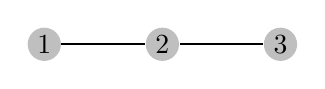
\begin{tikzpicture}[scale=1.5]
    % Draw a 7,11 network
    % First we draw the vertices
    \foreach \pos/\name in {{(1,0)/1}, {(2,0)/2}, {(3,0)/3}}
        \node[vertex] (\name) at \pos {$\name$};
    % Connect vertices with edges 
    \foreach \source/ \dest in {1/2, 2/3}
        \path[edge] (\source) -- (\dest) ;
        
\end{tikzpicture}
\end{center}

\begin{itemize}
\item At 1st period
\begin{itemize}
\item Rebel 2 chooses $\textbf{revolt}$ if he observes $\theta=(Rebel,Rebel,Rebel)$; Otherwise, chooses $\textbf{stay}$ forever.
\item Rebel 1 (or Rebel 3) choose \textbf{stay}.
\end{itemize}

\item After 1st period
\begin{itemize}
\item If Rebel 2 chooses \textbf{revolt} in the last period, then Rebel 1 (or Rebel 3) chooses \textbf{revolt} forever; 
\item If Rebel 2 chooses \textbf{stay} in the last period, then Rebel 1 (or Rebel 3) chooses \textbf{stay} forever.
\end{itemize}
 
 \item Any deviation $\Rightarrow$
 \begin{itemize}
 \item Choosing \textbf{stay} forever.
 \end{itemize}
\end{itemize}

  
}


\frame{
  \frametitle{Goal}

\textbf{Goal}

Can we generalize the result in Leading Example for all FFCCU networks?



}

\frame{
  \frametitle{Results}

\textbf{Results}
\begin{itemize}
\item $k=n$: we can.
\item $k<n$: with additional assumption,
\begin{itemize}
\item acyclic FFCCU: we can .
\item FFCCU: open question.
\end{itemize}
\end{itemize}

}


\frame{
  \frametitle{Result: $k=n$}

\begin{theorem}

\textbf{In} any FFCCU network, \textbf{if}  the prior has full support, \textbf{then} for repeated $k=n$ Threshold game, \textbf{there is} a $\delta$ such that a sequential equilibrium which is APEX \textbf{exists}.
\end{theorem}

Proof:
  \begin{enumerate}
  

  \item Some Inerts neighbors $\Rightarrow$ play \textbf{stay} forever.
  \item No Inert neighbor $\Rightarrow$ play \textbf{revolt} until \textbf{stay} is observed, and then play \textbf{stay} forever.
  \item Any deviation $\Rightarrow$ play \textbf{stay} forever.
  \item Since networks are FFCCU, there is a finite time $T^{\theta}$ such that ex-post efficient outcome repeats afterwards.

   \end{enumerate}

}

\frame{
  \frametitle{Result: $k=n$}

Comments:
\begin{enumerate}
\item \textbf{stay} $\Leftrightarrow$ some Inerts is observed.
\item single-period $\{\textbf{revolt}, \textbf{stay}\}$ $\Rightarrow$ reveals $\{\text{``no Inert'', ``some Inerts''}\}$.
\item Any deviation $\Rightarrow$ punished by shifting to \textbf{stay} forever by single player
\begin{itemize}
\item Group punishment is not necessary.
\end{itemize}
\end{enumerate}
}


\begin{frame}
  \frametitle{Result and Conjecture: $k<n$}


\begin{definition}
\textbf{Strong connectedness}$\Leftrightarrow$ for every pair of Rebels, there is a path consisting of Rebels to connect them.
\end{definition}  

\begin{definition}
\textbf{Full support on strong connectedness}$\Leftrightarrow$ 
\[\text{$\pi(\theta)>0$ if and only if $\theta$ has strong connectedness.}\]


\end{definition}  

\end{frame}





\begin{frame}
  \frametitle{Result and Conjecture: $k<n$}



\begin{theorem}
\label{thm_main_result}
\textbf{In} any {acyclic} FFCCU network, \textbf{if} {$\theta$ has strong connectedness} and \textbf{if} $\pi$ has full support  {on strong connectedness}, \textbf{then} for repeated $k<n$ Threshold game, \textbf{there is} a $\delta$ such that a {weak} sequential equilibrium which is APEX \textbf{exists}.
\end{theorem}

\begin{conjecture}
\textbf{In} any FFCCU network, ...[same as above]...
\end{conjecture}

\end{frame}

\section{Equilibrium construction}
\subsection{Equilibrium construction}

\frame{
  \frametitle{Equilibrium Construction: $k<n$}
\framesubtitle{Outline}

Outline

\begin{enumerate}
\item The role of Strong Connectedness
\item Communication by actions
\item Communication in equilibrium
\begin{enumerate}
\item Step 0: Build communication protocol
\item Step 1: Characterize ``information hierarchy'' in communication.
\item Step 2: Build reporting and coordination messages in the path, and characterize the in-path belief updating.
\item Step 3: Set up off-path belief.
\end{enumerate}

\end{enumerate}

}



\begin{frame}
   \frametitle{Equilibrium Construction: $k<n$}


\textbf{The role of Strong Connectedness}: 
\begin{itemize}
\item Otherwise, the game is reduced to incomplete information game without communication for some $\theta$
\end{itemize}

Example,
\begin{enumerate}


\item Let $k=2$. Assume $\theta=(Rebel_1,Inert_2,Rebel_3)$.
\item Let 
\begin{center}
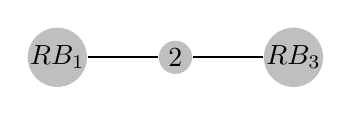
\begin{tikzpicture}[scale=1.5]
    % Draw a 7,11 network
    % First we draw the vertices
    \foreach \pos/\name in {{(1,0)/RB_1}, {(2,0)/2}, {(3,0)/RB_3}}
        \node[vertex] (\name) at \pos {$\name$};
    % Connect vertices with edges 
    \foreach \source/ \dest in {RB_1/2, 2/RB_3}
        \path[edge] (\source) -- (\dest) ;
        
\end{tikzpicture}
\end{center}
\item Then, Inert 2 block the information transmission.
\item This is an incomplete information game without communication.





\end{enumerate}
 




\end{frame}


\begin{frame}
  \frametitle{Equilibrium Construction: $k<n$}

\textbf{Communication by actions}
\begin{enumerate}


\item Indexing each node $i$ as a distinct prime number $x_i$. For instance,
\begin{center} 
  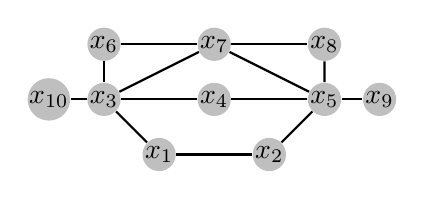
\begin{tikzpicture}[scale=0.7]
    % First we draw the vertices
    \foreach \pos/\name in {{(2,1)/x_1}, {(4,1)/x_2}, {(1,2)/x_3}, {(5,2)/x_5}, {(3,3)/x_7}, {(3,2)/x_4}, {(1,3)/x_6}, {(5,3)/x_8}, {(6,2)/x_9}, {(0,2)/x_{10}}}
        \node[vertex] (\name) at \pos {$\name$};
        
%        \foreach \pos/\name in {{(3,2)/4_L}, {(1,3)/6_L}, {(5,3)/8_L}, {(6,2)/9_L}, {(0,2)/10_L}}
%   \node[selected vertex] (\name) at \pos {$\name$};
    
    % Connect vertices with edges 
    \foreach \source/ \dest in {x_1/x_2, x_1/x_3, x_2/x_5, x_3/x_4, x_3/x_6, x_3/x_7, x_4/x_5, x_5/x_7, x_5/x_8, x_5/x_9,x_6/x_7, x_7/x_8, x_3/x_{10}}
        \path[edge] (\source) -- (\dest) ;
\end{tikzpicture}
\end{center} 
\item Then, for instance,
\begin{itemize}
\item If
\begin{center} 
  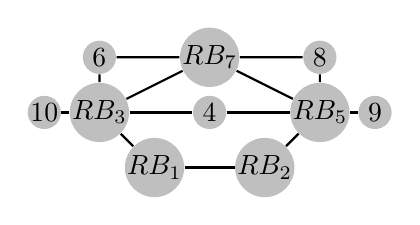
\begin{tikzpicture}[scale=0.7]
    % First we draw the vertices
    \foreach \pos/\name in {{(2,1)/RB_1}, {(4,1)/RB_2}, {(1,2)/RB_3}, {(5,2)/RB_5}, {(3,3)/RB_7}, {(3,2)/4}, {(1,3)/6}, {(5,3)/8}, {(6,2)/9}, {(0,2)/10}}
        \node[vertex] (\name) at \pos {$\name$};
        
%        \foreach \pos/\name in {{(3,2)/4_L}, {(1,3)/6_L}, {(5,3)/8_L}, {(6,2)/9_L}, {(0,2)/10_L}}
%   \node[selected vertex] (\name) at \pos {$\name$};
    
    % Connect vertices with edges 
    \foreach \source/ \dest in {RB_1/RB_2, RB_1/RB_3, RB_2/RB_5, RB_3/4, RB_3/6, RB_3/RB_7, 4/RB_5, RB_5/RB_7, RB_5/8, RB_5/9,6/RB_7, RB_7/8, RB_3/10}
        \path[edge] (\source) -- (\dest) ;
\end{tikzpicture}
\end{center} 

\item Rebel 3 report $x_1\times x_7 \times x_3$ to Rebel 1 by sending a finite sequence 
\[\textbf{stay},...,\textbf{stay},\underbrace{\textbf{revolt},\textbf{stay},...,\textbf{stay}}_{x_1\times x_7 \times x_3}\]
\end{itemize}

\end{enumerate}


\end{frame}








\begin{frame}
  \frametitle{Equilibrium Construction: $k<n$}

\textbf{Communication in Equilibrium. Step 0}
\begin{itemize}
\item Characterize the time horizontal line as 
\[\underbrace{\langle\text{coordination period}\rangle}_{0-block}\underbrace{\langle\text{reporting period}\rangle \langle\text{coordination period}\rangle}_{1-block}...\]

\begin{enumerate}
\item Reporting period: talking about $\theta$
\item Coordination period: talking about ``Have some Rebels known $\#[Rebels](\theta)\geq k$ or $\#[Rebels](\theta)< k$?'' 
\item Why do I need coordination period?
\end{enumerate}


\end{itemize}


\end{frame}


\begin{frame}
  \frametitle{Equilibrium Construction: $k<n$}

\textbf{Communication in Equilibrium. Step 0. }
\begin{itemize}
\item Q: Why do I need coordination period?
\item A: Since higher-order belief is hard to track.

\begin{itemize}
\item APEX: $T^{\theta}$ for all $\theta$.
\item Calculating $T^{\theta}$ for all $\theta$ is tedious.
\end{itemize}
\item I: If a Rebel knows $\#[Rebels](\theta)\geq k$ or $\#[Rebels](\theta)< k$ $\Rightarrow$ sending messages to let others know.
\end{itemize}


\end{frame}








\subsection{Information Hierarchy}

\begin{frame}
   \frametitle{Information Hierarchy}


Why do I need ``Information Hierarchy''?
\begin{itemize}
\item $\Rightarrow$ To ease the punishment scheme.
\item Case 1: \item Let $k=4$
\begin{center}
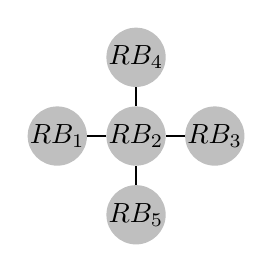
\begin{tikzpicture}[scale=1]
    % Draw a 7,11 network
    % First we draw the vertices
    \foreach \pos/\name in {{(1,1)/RB_1}, {(2,1)/RB_2}, {(3,1)/RB_3}, {(2,2)/RB_4}, {(2,0)/RB_5}}
        \node[vertex] (\name) at \pos {$\name$};
    % Connect vertices with edges 
    \foreach \source/ \dest in {RB_1/RB_2, RB_2/RB_3, RB_4/RB_2, RB_2/RB_5}
        \path[edge] (\source) -- (\dest) ;
        
\end{tikzpicture}
\end{center}

\begin{enumerate}
\item Rebel 1 can only be monitored by Rebel 2.
\item Given some strategies, suppose Rebel 2,3,4,5 can coordinate at period $T$ and play \textbf{revolt} forever.
\item If Rebel 1 deviate at period $T-1$, Rebel 2 has no incentive to punish him.
\end{enumerate}

\end{itemize}



\end{frame}


\begin{frame}
   \frametitle{Information Hierarchy}


Why do I need ``Information Hierarchy''?
\begin{itemize}
\item $\Rightarrow$ To characterize Rebels' incentives in communication.
\item Case 2: \item Let $k=4$
 \begin{center}
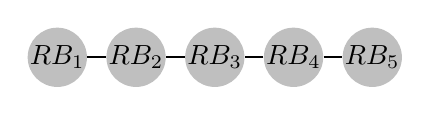
\begin{tikzpicture}[scale=1]
    % Draw a 7,11 network
    % First we draw the vertices
    \foreach \pos/\name in {{(1,1)/RB_1}, {(2,1)/RB_2}, {(3,1)/RB_3}, {(4,1)/RB_4}, {(5,1)/RB_5}}
        \node[vertex] (\name) at \pos {$\name$};
    % Connect vertices with edges 
    \foreach \source/ \dest in {RB_1/RB_2, RB_2/RB_3, RB_4/RB_3, RB_4/RB_5}
        \path[edge] (\source) -- (\dest) ;
        
\end{tikzpicture}
\end{center}

\begin{enumerate}
\item Rebel 2 has more incentive than Rebel 1 in sending messages.
\item Compare Rebel 3 and Rebel 2, etc.
\end{enumerate}

\end{itemize}



\end{frame}











\begin{frame}
  \frametitle{Information Hierarchy}

At $0$-block, let
  \begin{itemize}
  \item \[R^0=[Rebels](\theta)\]
  \end{itemize}


\end{frame}



\begin{frame}
  \frametitle{Information Hierarchy}

At $1$-block, let
\begin{eqnarray*}
N^0_i & \equiv &  G_i\\
I^0_i & \equiv & G_i\cap R^0\\
\end{eqnarray*}

Define $\leq^0$ by
\[i\in \leq^0 \Leftrightarrow \exists  j\in \bar{G}_i (I^0_i\subseteq N^0_j\cap R^0)\] 


Let 
\begin{eqnarray*}
R^{1} \equiv \{i\in R^0|i\notin \leq^0\}
\end{eqnarray*}




\end{frame}

\begin{frame}
  \frametitle{Information Hierarchy}

Ex., Rebel 1 is a non-$R^1$ node. Rebel 2 is a $R^1$ node. 

 \begin{center}
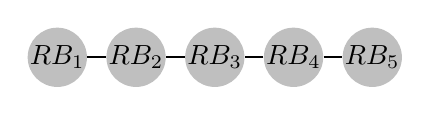
\begin{tikzpicture}[scale=1]
    % Draw a 7,11 network
    % First we draw the vertices
    \foreach \pos/\name in {{(1,1)/RB_1}, {(2,1)/RB_2}, {(3,1)/RB_3}, {(4,1)/RB_4}, {(5,1)/RB_5}}
        \node[vertex] (\name) at \pos {$\name$};
    % Connect vertices with edges 
    \foreach \source/ \dest in {RB_1/RB_2, RB_2/RB_3, RB_4/RB_3, RB_4/RB_5}
        \path[edge] (\source) -- (\dest) ;
        
\end{tikzpicture}
\end{center}

Calculation:

\begin{table}[h]
\begin{tabular}{l l}
$I^0_1=\{1,2\} $ &  $N^0_1\cap R^0=\{1,2\}$  \\
$I^0_2=\{1,2,3\}$ & $N^0_2\cap R^0=\{1,2,3\} $  \\
$I^0_3=\{2,3,4\}$ & $N^0_3\cap R^0=\{2,3,4\}$    \\
 &  
\end{tabular}
\end{table}

Main idea:
\begin{itemize}
\item Rebel 2 is more ``important'' than Rebel 1.
\item Rebel 3 and Rebel 2 are equally ``important'', etc.
\end{itemize}


\end{frame}





\begin{frame}
  \frametitle{Information Hierarchy}

In $t+1$-block, denote
\begin{eqnarray*}
N^t_i & \equiv & \bigcup_{k\in I^{t-1}_i}G_k \\
I^t_i & \equiv & \bigcup_{k\in G_i\cap R^t}I^{t-1}_k
\end{eqnarray*}
\begin{itemize}
\item $N^t_i$ is $i$'s \textit{extended} neighborhood given $i$'s information $I^{t-1}_i$
\item $I^t_i$ is $i$'s \textit{extended} Rebel neighbors given $j$'s information $I^{t-1}_j$, where $j$ is a $R^{t}$ Rebel. 
\end{itemize}


Define $\leq^t$ by
\[i\in \leq^t \Leftrightarrow \exists j\in \bar{G}_i(I^t_i\subseteq N^t_j\cap R^0)\] 


Let 
\begin{eqnarray*}
R^{t+1} \equiv  \{i\in R^t|i\notin \leq^t\}
\end{eqnarray*}


\end{frame}

\begin{frame}
  \frametitle{Information Hierarchy}

Ex.,
\begin{itemize}
\item Rebel 1 is a non-$R^1$ node. Rebel 2 is a $R^1$ node. Rebel 3 is a $R^1$ node.
\item Rebel 1 is a non-$R^2$ node. Rebel 2 is a non-$R^2$ node. Rebel 3 is a $R^2$ node.

\end{itemize}



\begin{center}
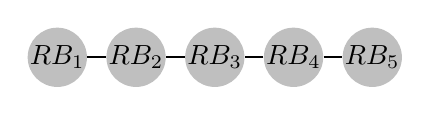
\begin{tikzpicture}[scale=1]
    % Draw a 7,11 network
    % First we draw the vertices
    \foreach \pos/\name in {{(1,1)/RB_1}, {(2,1)/RB_2}, {(3,1)/RB_3}, {(4,1)/RB_4}, {(5,1)/RB_5}}
        \node[vertex] (\name) at \pos {$\name$};
    % Connect vertices with edges 
    \foreach \source/ \dest in {RB_1/RB_2, RB_2/RB_3, RB_4/RB_3, RB_4/RB_5}
        \path[edge] (\source) -- (\dest) ;
        
\end{tikzpicture}
\end{center}

Calculation:

\begin{table}[h]
\begin{tabular}{l l}
at 1-block &    \\
\hline
$I^0_1=\{1,2\} $ &  $N^0_1\cap R^0=\{1,2\}$  \\
$I^0_2=\{1,2,3\}$ & $N^0_2\cap R^0=\{1,2,3\} $  \\
$I^0_3=\{2,3,4\}$ & $N^0_3\cap R^0=\{2,3,4\}$    \\
&    \\

at 2-block &    \\
\hline
$I^1_1=\{1,2,3\} $ &  $N^1_1\cap R^0=\{1,2,3\}$  \\
$I^1_2=\{1,2,3,4\}$ & $N^1_2\cap R^0=\{1,2,3,4\} $  \\
$I^1_3=\{1,2,3,4,5\}$ & $N^1_3\cap R^0=\{1,2,3,4,5\}$    \\
\end{tabular}
\end{table}


\end{frame}


\begin{frame}
  \frametitle{Information Hierarchy}


\begin{theorem}
\label{lemma_empty}
Given $\theta$, if the network is FFCCU and acyclic and if the state has strong connectedness $\Rightarrow$ $\exists t^{\theta}$ such that some $R^{t^{\theta}}$ Rebels whose $I^{t^{\theta}}\supset [Rebels](\theta)$.
\end{theorem} 
\end{frame}










\section{Equilibrium path}
\begin{frame}
\frametitle{Equilibrium path}

At $t$-block, looking for messages (strategies) such that
\begin{itemize}
\item The length of players' messages is the same as the length of corresponding period.   
\item $RP^t$: the reporting period

\[\overbrace{\langle \cdot \cdot \cdot \rangle}^{\text{\small reporting period}}\] 

\item $CD^t$: the coordination period

\[\overbrace{\langle\underbrace{\langle \text{\tiny sub-block} \rangle \cdot \cdot \cdot \langle \cdot \rangle}_{\text{division}}\rangle \langle\underbrace{\langle \cdot \rangle \cdot \cdot \cdot \langle \cdot \rangle}_{\text{division}} \rangle \langle\underbrace{\langle \cdot \rangle \cdot \cdot \cdot \langle \cdot \rangle}_{\text{division}}\rangle}^{\text{\small coordination period}}\] 

\item $\langle RP^t \rangle$: the reporting messages
\item $\langle CD^t \rangle$: the coordination messages

\end{itemize}



\end{frame}


\begin{frame}
\frametitle{Equilibrium path}

Denote
\begin{itemize}
\item $\langle I^{t-1}_i\rangle$=$\textbf{s},...,\textbf{s},\underbrace{\textbf{r},\textbf{s},...,\textbf{s}}_{X}$
\begin{itemize}
\item $X=\times_{j\in I^{t-1}_i}\text{ j's prime index}$
\end{itemize}
\item $\langle \textbf{stay} \rangle$=$\textbf{s},...,\textbf{s}$
\end{itemize}

Ideally, (by information hierarchy theory),
\begin{itemize}
\item $R^t$: report $\langle I^{t-1} \rangle$.
\item Non-$R^t$: report $\langle \textbf{stay} \rangle$.
\item $\Rightarrow$ some Rebels knows the state.
\end{itemize}


\end{frame}

\begin{frame}
\frametitle{Equilibrium path}

However, not so obvious. 
\begin{itemize}
\item Not cheap talks.
\item Consider next 3 problems, where we suppose
\begin{itemize}
\item An action-irrelevant message $\langle M \rangle$.
\item Starting with a $RP$ and then a $CD$ follows. 
\item Observing $\langle M \rangle$ in $CD$ $\Rightarrow$ play \textbf{revolt} forever; Otherwise $\Rightarrow$ play \textbf{stay} forever.
\end{itemize}
\end{itemize}



\end{frame}


\begin{frame}
\frametitle{Equilibrium path}

\textbf{Pivotal player case 1: Free Rider Problem}. (Rebel 4 and Rebel 5)

\begin{itemize}
\item $k=5$


\end{itemize}

\begin{center}
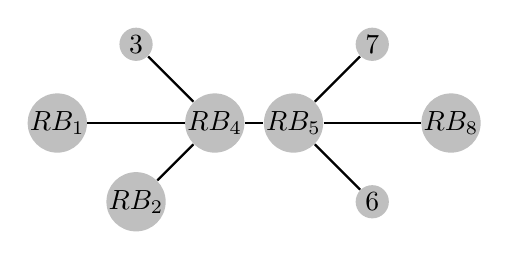
\begin{tikzpicture}[scale=1]
    % Draw a 7,11 network
    % First we draw the vertices
    \foreach \pos/\name in {{(1,2)/RB_1}, {(2,1)/RB_2}, {(2,3)/3}, {(3,2)/RB_4}, {(4,2)/RB_5}, {(5,1)/6}, {(5,3)/7}, {(6,2)/RB_8}}
        \node[vertex] (\name) at \pos {$\name$};
    
    
    % Connect vertices with edges 
    \foreach \source/ \dest in {RB_1/RB_4, RB_2/RB_4,3/RB_4,RB_4/RB_5, RB_5/6, RB_5/7, RB_5/RB_8}
        \path[edge] (\source) -- (\dest) ;
        
\end{tikzpicture}
\end{center}

\begin{itemize}
\item \textbf{Problem}: Both Rebel 4 and Rebel 5 are pivotal $\Rightarrow$ they will shift to play $\langle \textbf{stay} \rangle$ if others report truthfully.
\end{itemize}


\end{frame}


\begin{frame}
\frametitle{Equilibrium path}

\textbf{Pivotal Player Case 2} (Rebel 5)

\begin{itemize}
\item $k=6$

\end{itemize}

\begin{center}
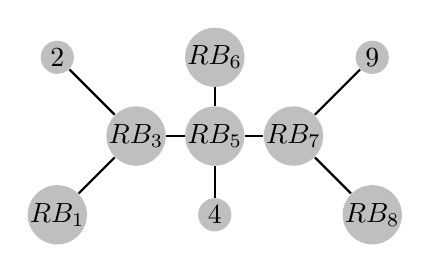
\begin{tikzpicture}[scale=1]
    % Draw a 7,11 network
    % First we draw the vertices
    \foreach \pos/\name in {{(1,1)/RB_1}, {(1,3)/2}, {(2,2)/RB_3}, {(3,1)/4}, {(3,2)/RB_5}, {(3,3)/RB_6}, {(4,2)/RB_7}, {(5,1)/RB_8}, {(5,3)/9}}
        \node[vertex] (\name) at \pos {$\name$};
    
    
    % Connect vertices with edges 
    \foreach \source/ \dest in {RB_1/RB_3, 2/RB_3,RB_3/RB_5,4/RB_5, RB_6/RB_5, RB_5/RB_7, RB_7/RB_8, RB_7/9}
        \path[edge] (\source) -- (\dest) ;
        
\end{tikzpicture}
\end{center}

\begin{itemize}
\item \textbf{Problem}: Rebel 5 is pivotal $\Rightarrow$ he shifts to play $\langle \textbf{stay} \rangle$ given others' truthful reporting.
\end{itemize}

\end{frame}

\begin{frame}
\frametitle{Equilibrium path}

\textbf{Pivotal Player Case 3} (Rebel 4)

\begin{itemize}
\item $k=6$


\end{itemize}

\begin{center}
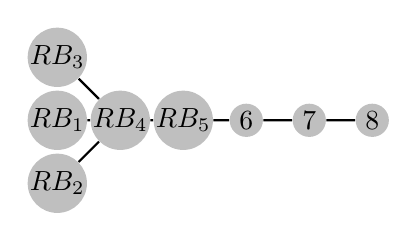
\begin{tikzpicture}[scale=0.8]
    % Draw a 7,11 network
    % First we draw the vertices
    \foreach \pos/\name in {{(2,2)/RB_1}, {(2,1)/RB_2}, {(2,3)/RB_3}, {(3,2)/RB_4}, {(4,2)/RB_5}, {(5,2)/6}, {(6,2)/7}, {(7,2)/8}}
        \node[vertex] (\name) at \pos {$\name$};
    
    
    % Connect vertices with edges 
    \foreach \source/ \dest in {RB_1/RB_4, RB_2/RB_4,RB_3/RB_4,RB_4/RB_5, RB_5/6, 6/7, 7/8}
        \path[edge] (\source) -- (\dest) ;
        
\end{tikzpicture}
\end{center}

\begin{itemize}
\item \textbf{Problem}: Rebel 4 is pivotal $\Rightarrow$ he shifts to play $\langle \textbf{stay} \rangle$ given others' truthful reporting.
\end{itemize}

\end{frame}


\begin{frame}
\frametitle{Equilibrium path}

Problem
\begin{itemize}
\item Rebels may deviate $\langle I^{t-1} \rangle$ to $\langle \textbf{stay} \rangle$.
\end{itemize}

Remedy
\begin{itemize}
\item $\langle 1 \rangle= \textbf{s},...,\textbf{s},\textbf{r}$, as the message used by pivotal player.
\item Continuation behavior contingent on both $RP$ and $CD$.

\end{itemize}

Good news. 
\begin{itemize}
\item Pivotal problems: only above three cases.
\item The free rider problem: only the above case.
\begin{itemize}
\item Two nearby Rebels. (only for acyclic $G$)
\end{itemize}

\end{itemize}

\end{frame}





\begin{frame}
\frametitle{Equilibrium path}

Good news
\begin{itemize}
\item With suitable coordination messages and continuation behavior
\begin{enumerate}
\item Pivotal players will not deviate from playing $\langle 1 \rangle$.
\item Only pivotal players will play $\langle 1 \rangle$
\end{enumerate}


\end{itemize}


\end{frame}


\begin{frame}
\frametitle{Equilibrium path}

Good news
\begin{itemize}
\item By adding a $\langle \mathbf{x}_i \rangle=\textbf{s},...,\textbf{s},\underbrace{\textbf{r},\textbf{s},...,\textbf{s}}_{x_i}$.
\begin{itemize}
\item To create more equilibrium paths in coordination period.
\end{itemize}
\item The belief updating after $CD^t$, $t>0$ in the equilibrium path will be

\end{itemize}


\begin{table}[ht]
\caption{Belief updating after $CD^t$, $t>0$}
\label{Table_blf_up_cdt12}
\begin{center}
\begin{tabular}{l c c c}
In $RP^t$ 	 	&  	In $CD^t_{1,1}$		&  In $CD^t_{1,2}$	  &\\
\hline
\hline
$i$ plays 		                             &  	$i$ plays		&				$i$ plays			& The events $j$ believe with probability one  \\
\hline
$\langle  \textbf{stay} \rangle$ 	& 	$\langle \mathbf{x}_i \rangle$	&  $\langle \textbf{stay} \rangle$ &  $i\notin R^t$ \\
$\langle  {I^{t-1}_i} \rangle$ 		&  $\langle \textbf{stay} \rangle$	&	$\langle \textbf{stay} \rangle$ &  $\#[Rebels](\theta)< k$   \\
$\langle  {I^{t-1}_i} \rangle$ 		&  $\langle \mathbf{x}_i \rangle$	&	$\langle \textbf{stay} \rangle$ &  $\#[Rebels](\theta)\geq k$    \\
$\langle  {I^{t-1}_i} \rangle$ 		&  $\langle \mathbf{x}_i \rangle$	&	$\langle \mathbf{x}_i \rangle$ &  $i\in R^t$  \\
$\langle 1 \rangle$ 		             &  $\langle \textbf{stay} \rangle$	&	$\langle \textbf{stay} \rangle$ &  $\#[Rebels](\theta)< k$\\
$\langle 1 \rangle$ 		             &  $\langle \mathbf{x}_i \rangle$	&	$\langle \textbf{stay} \rangle$ & $\#[Rebels](\theta)\geq k$
\end{tabular}
\end{center}
\end{table}

\end{frame}


\begin{frame}
\frametitle{Off-path Belief}

$i$ detects a deviation at $s$ period, he forms off-path belief
\begin{equation}
\label{eq_grim_trigger}
\sum_{\theta \in \{\theta:\theta_j=Inert,j\notin G_i\}}\beta^{\pi,\tau}_{G_i}({\theta}|h^{s^{'}}_{G_i})=1
\end{equation}
for all $s^{'}\geq s$. 

\begin{enumerate}
\item If $\# I^0_i<k$, he will play \textbf{stay} forever.
\item This off-path belief then serve as a grim trigger.
\end{enumerate}




\end{frame}


\begin{frame}
\frametitle{Off-path Belief}

Without $\langle 1 \rangle$, using this grim-trigger-like belief may not sustain APEX
\begin{itemize}
\item $k=5$

\end{itemize}

\begin{center}

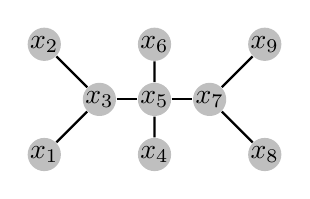
\begin{tikzpicture}[scale=0.7]
    % Draw a 7,11 network
    % First we draw the vertices
    \foreach \pos/\name in {{(1,1)/x_1}, {(1,3)/x_2}, {(2,2)/x_3}, {(3,1)/x_4}, {(3,2)/x_5}, {(3,3)/x_6}, {(4,2)/x_7}, {(5,1)/x_8}, {(5,3)/x_9}}
        \node[vertex] (\name) at \pos {$\name$};
    
    
    % Connect vertices with edges 
    \foreach \source/ \dest in {x_1/x_3, x_2/x_3,x_3/x_5,x_4/x_5, x_6/x_5, x_5/x_7, x_7/x_8, x_7/x_9}
        \path[edge] (\source) -- (\dest) ;
        
\end{tikzpicture}

\end{center}

\begin{center}
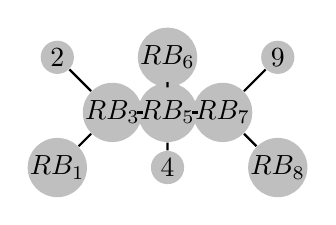
\begin{tikzpicture}[scale=0.7]
    % Draw a 7,11 network
    % First we draw the vertices
    \foreach \pos/\name in {{(1,1)/RB_1}, {(1,3)/2}, {(2,2)/RB_3}, {(3,1)/4}, {(3,2)/RB_5}, {(3,3)/RB_6}, {(4,2)/RB_7}, {(5,1)/RB_8}, {(5,3)/9}}
        \node[vertex] (\name) at \pos {$\name$};
    
    
    % Connect vertices with edges 
    \foreach \source/ \dest in {RB_1/RB_3, 2/RB_3,RB_3/RB_5,4/RB_5, RB_6/RB_5, RB_5/RB_7, RB_7/RB_8, RB_7/9}
        \path[edge] (\source) -- (\dest) ;
        
\end{tikzpicture}
\end{center}

\begin{itemize}
\item \textbf{Problem}: Without $\langle 1 \rangle$ being considered as an in-path strategies; 
\item Rebel 4 is pivotal; He shifts to report $x_3\times x_5 \times x_7$ instead of $x_3\times x_5 \times x_7 \times x_6$. 
\item Coordination can be made, but Rebel 6 is out of coordination since he detects a deviation.
\end{itemize}

\end{frame}


\frame{
  \frametitle{Result: $k<n$}

Comments:
\begin{enumerate}
\item \textbf{stay} $\not\Leftrightarrow$ some Inerts be observed.
\item single-period $\{\textbf{revolt}, \textbf{stay}\}$ $\not\Rightarrow$ reveals $\{\#[Rebels](\theta)\}$
\item Any deviation $\Rightarrow$ punished by shifting to \textbf{stay} forever by some players.

\end{enumerate}
}




\begin{frame}
\frametitle{Discussion}

\begin{enumerate}


\item From the above steps, an APEX equilibrium is constructed.
\item We can relaxed the assumption that payoff is hidden.
\begin{itemize}
\item payoff is perfectly observed: easy to construct an APEX equilibrium.
\item payoff is noisy: with full support assumption, the existing equilibrium is APEX
\end{itemize}
\item This proof is still open for FFCCU network with cycles.
\item Off-path belief did not satisfy full consistency property for FFCCU network without cycles.

\item Prime number indexing also works for other discreet and finite state space.


\end{enumerate}


\end{frame}




\begin{frame}

\frametitle{Conclusion}


\begin{enumerate}
\item I show that, without cheap talk, in this repeated $k$-threshold game played in FFCCU networks without cycles, coordination still can happen.
\begin{itemize}
\item Using sequence of actions to communicate.
\end{itemize}
\item The equilibrium is constructive and does not rely on public or private signals other than actions.
\item We can use prime number to index the states given that states are discrete and finite.
\item For the network with circle, it is still remaining to tackle with.
\end{enumerate}
\end{frame}










\end{document}
